\documentclass{standalone}
\usepackage{tikz}
\usetikzlibrary{shapes.geometric}

\begin{document}
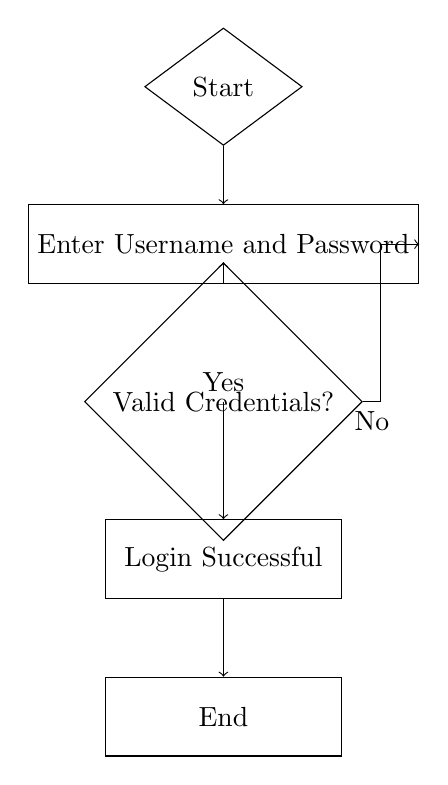
\begin{tikzpicture}[node distance=2cm]
  % Define start node (diamond)
  \node (start) [diamond, draw, minimum width=2cm, minimum height=0.8cm] {Start};
  
  % Define input node (rectangle)
  \node (input) [below of=start, rectangle, draw, minimum width=3cm, minimum height=1cm] {Enter Username and Password};
  
  % Define decision node (diamond)
  \node (decision) [below of=input, diamond, draw, minimum width=2cm, minimum height=0.8cm] {Valid Credentials?};
  
  % Define process node (rectangle)
  \node (process) [below of=decision, rectangle, draw, minimum width=3cm, minimum height=1cm] {Login Successful};
  
  % Define end node (rectangle)
  \node (end) [below of=process, rectangle, draw, minimum width=3cm, minimum height=1cm] {End};
  
  % Draw arrows between nodes
  \draw[->] (start) -- (input);
  \draw[->] (input) -- (decision);
  \draw[->] (decision) -| node[near start, above] {Yes} (process);
  \draw[->] (decision) -| node[near start, below] {No} ++(2,0) |- (input); % Assuming loop back to input if credentials are invalid
  
  \draw[->] (process) -- (end);
\end{tikzpicture}
\end{document}